%%%%%%%%%%%%%%%%%%%%%%%%%%%%%%%%%%%%%%%%%%%%%%%%%%%%%%%%%%%%%%%%%%%%%%%%%%%%%%%%
%2345678901234567890123456789012345678901234567890123456789012345678901234567890
%        1         2         3         4         5         6         7         8

\documentclass[letterpaper, 10 pt, conference]{ieeeconf}  % Comment this line out if you need a4paper
\usepackage[portuguese]{babel}
%\documentclass[a4paper, 10pt, conference]{ieeeconf}      % Use this line for a4 paper

\IEEEoverridecommandlockouts                              % This command is only needed if 
                                                          % you want to use the \thanks command

\overrideIEEEmargins                                      % Needed to meet printer requirements.

% See the \addtolength command later in the file to balance the column lengths
% on the last page of the document


% The following packages can be found on http:\\www.ctan.org
\usepackage{graphics} % for pdf, bitmapped graphics files
\usepackage{epsfig} % for postscript graphics files
\usepackage{mathptmx} % assumes new font selection scheme installed
\usepackage{times} % assumes new font selection scheme installed
\usepackage{amsmath} % assumes amsmath package installed
\usepackage{amssymb}  % assumes amsmath package installed
\usepackage{subcaption}
\captionsetup{compatibility=false}
\usepackage{alltt}
\usepackage[noadjust]{cite}
\usepackage{float}
\usepackage{comment}
\usepackage{array}
\usepackage{makecell}
\usepackage[ruled,lined,linesnumbered]{algorithm2e}
\usepackage{flushend}
\usepackage[utf8]{inputenc}


\title{\LARGE \bf
Análise via Simulação dos Protocolos IEEE 802.11s e FLAME em Redes em Malha sem Fio
}


\author{Lucas de Carvalho Gomes% <-this % stops a space
\\Grupo de Teleinformática e Automação - PEE/COPPE
\\Universidade Federal do Rio de Janeiro (UFRJ)
\\gomes@gta.ufrj.br
}



\begin{document}
\selectlanguage{portuguese}


\maketitle
\thispagestyle{empty}
\pagestyle{empty}


%%%%%%%%%%%%%%%%%%%%%%%%%%%%%%%%%%%%%%%%%%%%%%%%%%%%%%%%%%%%%%%%%%%%%%%%%%%%%%%%
\begin{abstract}

Redes em malha sem-fio ou redes~\textit{mesh} têm sido adotadas como alternativas de baixo custo para implementar redes sem-fio de acesso á Internet. São caracterizadas por um \textit{backbone} de roteadores sem-fio, nos quais há pelo menos um ponto de acesso a redes externas, que trocam informações entre si, executando algoritmos de roteamento. As vantagens desta abordagem são o aumento no alcance e o baixo custo de instalação. Atualmente, há diversas propostas de algoritmos de roteamento, cada uma priorizando critérios diferentes. Este trabalho visa executar simulações de redes em malha através do popular simulador de redes \textit{ns-3} (\textit{The Network Simulator 3}). São comparadas duas abordagens para o roteamento: o padrão IEEE 802.11s e o protocolo FLAME (\textit{Forwarding Layer for Meshing}), de acordo com a taxa de entrega de pacotes, o atraso médio e o atraso da primeira transmissão.

\end{abstract}

\begin{keywords}
Redes em malha sem-fio, ns-3, IEEE 802.11s, FLAME
\end{keywords}

%%%%%%%%%%%%%%%%%%%%%%%%%%%%%%%%%%%%%%%%%%%%%%%%%%%%%%%%%%%%%%%%%%%%%%%%%%%%%%%%
\section{INTRODUÇÃO}
\label{sec:intro}

As redes em malha sem-fio são uma arquitetura de rede sem-fio que visa ampliar o alcance do acesso à Internet em uma determinada região. Para isto, redes em malha possuem um \textit{backbone}, ou seja, um conjunto de roteadores sem-fio cujas posições são fixas. Por meio do encaminhamento de quadros por múltiplos saltos, pode-se ampliar o alcance além do alcance de um único ponto de acesso sem-fio diretamente conectado à Internet. A presença de um conjunto de roteadores que não se movem torna possível utilizar métricas de roteamento elaboradas que levam em consideração a qualidade da transmissão no meio, que são denominadas métricas cientes da qualidade. Isto é uma vantagem em relação às redes sem-fio \textit{ad-hoc}, que, devido à mobilidade dos pontos de acesso, torna as informações da qualidade da conexão muito variáveis em relação ao tempo.

Redes \textit{mesh}, no entanto, também enfrentam alguns desafios. Um dos mais significativos é a presença de interferência intra-fluxo e inter-fluxos, que depende do arranjo dos roteadores do \textit{backbone}. A interferência intra-fluxo ocorre quando há quadros diferentes de uma mesma transmissão que colidem entre si durante o roteamento; a interferência inter-fluxos é a colisão de informações provenientes de transmissões (ou fluxos) diferentes. A ocorrência de colisões nestes dois cenários inicia mecanismos do método de controle de acesso ao meio. Por exemplo, no caso do CSMA/CA (\textit{Carrier Sense Multiple Access with Collision Avoidance}), utilizado no padrão IEEE 802.11, uma colisão faz com que as estações envolvidas tenham que aguardar um período de \textit{backoff}, que é aleatório. Com isto, estas colisões podem prejudicar a qualidade da conexão, devido aos seus impactos no atraso e na perda de pacotes. Além disto, a presença de múltiplas transmissões, além das colisões, causa uma espera maior no acesso ao meio, ou seja, mesmo sem colisões, a qualidade é prejudicada. Estes fatores tornam difícil garantir requisitos de Qualidade de Serviço (QoS - \textit{Quality of Service}).

A possibilidade de considerar a qualidade da transmissão e a presença dos desafios mencionados no parágrafo anterior motivaram a criação de diversos protocolos de roteamento e métricas para ponderar os enlaces sem-fio entre dois pontos de acesso. Neste trabalho, serão avaliadas, por meio de simulações, duas propostas para este cenário: o padrão IEEE 802.11s~\cite{carrano2011,hiertz2010,andreev2010} e o protocolo FLAME (\textit{Forwarding Layer for Meshing})~\cite{andreev2010,graaf2007}, implementadas no popular simulador de redes \textit{ns-3} (\textit{The Network Simulator 3})~\cite{ns3}, que serão descritos a seguir.

O restante do trabalho está organizado da seguinte forma: a Seção 2 descreve em detalhes as duas propostas consideradas neste cenário; a Seção 3 discorre sobre o cenário de simulação utilizado, as métricas consideradas e os parâmetros que foram ajustados; a Seção 4 exibe os resultados obtidos; por fim, a Seção 5 apresenta as conclusões deste trabalho.

\section{Abordagens Utilizadas}\label{sec:protocols}

\subsection{Padrão IEEE 802.11s}

O IEEE 802.11s é um adendo ao padrão IEEE 802.11, que define as camadas física e de enlace para redes sem-fio. Este adendo define o encaminhamento em múltiplos saltos para redes sem-fio, para o qual também foram necessárias algumas alterações na camada de enlace e na subcamada de controle de acesso ao meio (MAC - \textit{Medium Access Control}). Para este objetivo, também define mecanismos de descoberta de caminhos e manutenção de enlaces entre dois roteadores de um \textit{backbone}~\cite{carrano2011,hiertz2010,andreev2010}.

O padrão define uma arquitetura que separa as estações e roteadores participantes de uma rede \textit{mesh} em quatro categorias:

\begin{itemize}

	\item Cliente ou Estação (STA): um nó que apenas realiza requisições. Não participa dos algoritmos de descoberta de caminhos nem encaminha quadros.
    
    \item Pontos da Malha (\textit{Mesh Points} ou \textit{Mesh STAs}): participam do roteamento, mas não oferecem acesso aos clientes.
    
    \item Pontos de Acesso da Malha (\textit{Mesh Access Points}): participam do roteamento e fornecem acesso ás estações.
    
    \item Portais (\textit{Portals} ou \textit{Mesh Portal Points}): responsável por conectar a rede \textit{mesh} a redes externas. Assim como os pontos da malha, não são usados para oferecer acesso às estações.

\end{itemize}

A arquitetura não limita a quantidade de portais: é possível haver mais de um portal dentro da mesma rede em malha; neste caso, um cliente precisa definir por qual portal suas comunicações serão mantidas.

Cada rede em malha possui três elementos principais: um identificador, necessário para que os nós de uma mesma malha se reconheçam e para que seja possível realizar uma associação, um protocolo de criação de caminhos e uma métrica para escolher entre os caminhos disponíveis.

O identificador da malha é o campo \textit{Mesh ID}, um campo extra adicionado às sondas de anúncio de redes locais definidas no IEEE 802.11. Este campo é diferente do SSID (\textit{Service Set IDentifier}), usado para distinguir redes infraestruturadas convencionais.

Um ponto importante definido no IEEE 802.11s é um mecanismo de manutenção de enlaces entre pares (\textit{peers}), que correspondem às arestas em um grafo da malha; ou seja, um mecanismo para descoberta de vizinhos. Ele é executado por meio do PMP (\textit{Peer Management Protocol}), que prevê trocas de mensagens para o estabelecimento e para a remoção de um enlace. Para estabelecer um enlace, dois Pontos da Malha trocam mensagens do tipo \textit{Peer Link Open} e \textit{Peer Link Confirm}. Para que os enlaces sejam bidirecionais, esta troca é realizada nos dois sentidos. Para remover um enlace, um dos pontos deve enviar uma mensagem \textit{Peer Link Close}. Um enlace é identificado pelos endereços MAC dos dois participantes e por um par de identificadores do enlace, gerado por cada um dos mesmos. Além do mecanismo de encerrar conexões definido pelo padrão, a implementação do \textit{ns-3} define um procedimento adicional: duas heurísticas baseadas na perda de quadros de controle periódicos e na perda de quadros de dados transmitidos~\cite{andreevsite}. Dois limiares são estabelecidos, cada um para a quantidade de perdas consecutivas de um tipo de quadro. Quando um dos dois limiares é ultrapassado, o enlace é encerrado.

O IEEE 802.11s define um protocolo de seleção e descoberta de caminhos cuja instalação é mandatória: o HWMP (\textit{Hybrid Wireless Mesh Protocol}). O HWMP é um protocolo híbrido, ou seja, executa um método pró-ativo e um reativo de descoberta de caminhos, buscando explorar as vantagens das duas abordagens. Sua concepção é baseada no protocolo AODV (\textit{Ad-hoc On Demand Distance Vector}), um protocolo reativo para redes sem-fio \textit{ad-hoc} e na sua extensão AODV-ST (\textit{Ad-hoc On Demand Distance Vector -- Spanning Tree}), que adiciona a funcionalidade da manutenção de uma árvore que possui um portal como raiz por meio de uma inundação periódica.

O HWMP pode ser configurado para operar em dois modos: o modo reativo sob demanda, que estabelece um caminho entre um par qualquer de pontos da malha apenas quando ocorre uma transmissão entre os mesmos, e o modo pró-ativo, que emprega uma topologia baseada em árvores, calculada assim que um ponto da malha se anuncia como raiz da árvore. O encaminhamento em uma arquitetura baseada em árvores concentra todas as transmissões na raiz, que reenvia os quadros ao destino dos mesmos. Por isto, a árvore precisa manter uma tabela de roteamento contendo todos os possíveis destinos dentro da malha.

Cada modo de operação apresenta suas vantagens: o modo sob-demanda é útil para estabelecer caminhos quando não há um destino prioritário para o tráfego ou quando os pares envolvidos nas comunicações variam muito com o tempo. Já o modo pró-ativo é interessante quando há uma matriz de tráfego definida, ou seja, quando há tendência de encaminhar uma parte significativa do tráfego para alguns nós; um caso para isto é um Portal assumir o papel de raiz da árvore.

O HWMP é híbrido pois utiliza os dois mecanismos simultaneamente, o que permite utilizar as duas vantagens: a parcela de tráfego que é direcionada para um subconjunto de nós é favorecida pela árvore pré-estabelecida, e a parcela do tráfego que não possui um padrão definido pode utilizar o modo sob-demanda para não ser prejudicada por um caminho não-ótimo que envolve a transmissão à raiz e a retransmissão da raiz ao destino.

Para a descoberta de caminhos nos dois modos, o padrão define quatro tipos de quadros de controle:

\begin{itemize}
	\item \textit{Path Request} (PREQ): quadros transmitidos por um ponto da malha que necessita descobrir um caminho para outro ponto da malha;
    \item \textit{Path Reply} (PREP): quadros enviados em resposta a um PREQ a partir do destino da requisição ou, ocasionalmente, a partir de nós intermediários que conheçam um caminho ao destino;
    \item \textit{Path Error} (PERR): notificação de que um caminho não existe mais;
    \item \textit{Root Announcement} (RANN): transmitido pela raiz em difusão para anunciar-se na malha. Usado em um dos dois possíveis modos de operação pró-ativos.
\end{itemize}

Como mencionado na definição do RANN, há dois modos de operação pró-ativos: um utiliza uma troca de quadros PREQ e PREP, o outro utiliza uma difusão de um quadro RANN a partir da raiz e o envio de PREPs a partir de todos os outros nós da malha à raiz. Atualmente, a implementação do \textit{ns-3} só considera o modo PREQ/PREP~\cite{andreevsite}. Por isto, somente este será detalhado abaixo.

O procedimento funciona através dos passos abaixo:

\begin{itemize}
	\item A raiz transmite em difusão um quadro PREQ com os bits DO (\textit{Destination Only}) e RF (\textit{Respond and Forward}) ativos; assim, a retransmissão do PREQ só encerrará quando o destino for alcançado e cada nó intermediário enviará um PREP à raiz, permitindo que a raiz mantenha a sua tabela de roteamento;
    \item Nós intermediários retransmitem o PREQ recebido e enviam PREPs à raiz;
    \item O destino recebe o PREQ e envia um PREP à raiz;
\end{itemize}

A seguir, o procedimento reativo é descrito. Para isto, vamos supor que um nó $F$ deseje transmitir uma mensagem a outro nó da malha $D$. O funcionamento, então, se dará da seguinte forma:

\begin{itemize}
	\item $F$ transmite em difusão um PREQ;
    \item Nós intermediários, ao receberem o PREQ, verificam se já existe um caminho conhecido nas suas tabelas de roteamento. Caso haja, enviam PREPs de volta à raiz;
    \item Caso contrário, o PREQ continua sendo retransmitido até alcançar $D$;
    \item $D$ recebe o PREQ e envia um PREP à raiz;
\end{itemize}

A cada retransmissão de um PREQ ou PREP, nós intermediários e o destino atualizam o campo de Métrica presente no quadro. Assim, é possível determinar o custo dos caminhos, tanto na origem quanto no destino, e é possível escolher o melhor deles.

A métrica mandatória para ponderar os enlaces sem-fio é o \textit{Airtime} (em tradução livre, tempo no ar). Esta métrica estima o tempo que leva a transmissão de um quadro de teste, ou seja, por quanto tempo ele ocupa o meio. O protocolo definido pelo IEEE 802.11s visa minimizar esta métrica, ou seja, as transmissões devem seguir caminhos que ocupem o meio de transmissão pelo menor tempo possível. O seu cálculo leva em consideração a taxa de transmissão à qual o quadro é transmitido, a sobrecarga (ou \textit{overhead}) imposta pela implementação utilizada para a camada física e a probabilidade da ocorrência de uma retransmissão - ou seja, a probabilidade de perda de quadros, que é correlacionada com a taxa de erros em um enlace. O padrão não define	como é calculada a probabilidade de perda de quadros, deixando este detalhe para a implementação. O \textit{Airtime} é definido pela seguinte equação:
%
\begin{equation}
	c_a=\Big[O + \frac{B_t}{r}\Big] \frac{1}{1-e_f},
\end{equation}
%
na qual $O$ é uma constante que corresponde à latência imposta pelo \textit{overhead} da implementação da camada física, $B_t$ é o tamanho do quadro de testes (1024 bytes), $r$ é a taxa de transmissão em Mb/s na qual um ponto da malha transmite o quadro de testes e $e_f$ corresponde à probabilidade de perda do quadro de teste estimada. Os caminhos escolhidos com maior prioridade são os caminhos que contém os menores valores de \textit{Airtime}.

A métrica é calculada periodicamente pelos nós da rede, por meio da transmissão periódica dos quadros de controle para a descoberta de caminhos. Assim, o protocolo se ajusta a variações da qualidade da comunicação.

\subsection{FLAME}

FLAME (\textit{Forwarding Layer for Meshing}) é um protocolo que opera entre a camada de enlace e a camada de rede (também chamada de "camada 2.5"). Habilita o encaminhamento por múltiplos saltos utilizando endereços MAC e é totalmente transparente à camada de rede. FLAME não usa nenhum mecanismo de descoberta de rotas; para atualizar uma tabela de roteamento, um nó que opera neste protocolo analisa o tráfego recebido e realiza atualizações de acordo com as informações obtidas~\cite{andreev2010,graaf2007}.

O protocolo considera que uma premissa é válida: todos os enlaces são bidirecionais. Com isto, ele constrói uma tabela de roteamento baseado nos caminhos inversos tomados pelos quadros que um nó recebe. O protocolo também utiliza uma inundação periódica de quadros de dados. Para evitar repetições, cada quadro de dados carrega um número de sequência e as tabelas de roteamento armazenam os últimos números de sequência; desta forma, um quadro que carrega um número de sequência já recebido é descartado. A constante atualização e o uso de uma inundação periódica e controlada fazem com que os dados trafeguem por caminhos aleatórios e que mudam muito com o tempo. A intenção disto é maximizar a taxa de entrega de pacotes.

O procedimento para encaminhar quadros depende da origem dos mesmos. Para quadros gerados localmente, os passos são os seguintes:

\begin{itemize}
	\item Para quadros~\textit{broadcast} ou~\textit{multicast}, o endereço do próximo salto é configurado como o endereço de \textit{broadcast};
    \item Se houver um próximo salto definido para o seu destino na tabela de roteamento, o quadro será enviado para o seu endereço;
    \item Se não houver um próximo salto definido para este destino, o próximo salto é configurado como o endereço de \textit{broadcast};
    \item Caso a estação não tenha enviado quadros em difusão por mais de 5 segundos, o próximo salto é o endereço de \textit{broadcast}.
\end{itemize}

Os passos para quadros que devem ser retransmitidos são:

\begin{itemize}
	\item Verificar se o número de sequência do quadro é o mais recente, comparando-o com a entrada do emissor do quadro na tabela de roteamento;
    \item Se o endereço MAC de destino for \textit{unicast} e o próximo salto for desconhecido, o quadro é descartado. Caso contrário, o quadro é enviado para o próximo salto presente na tabela;
    \item Se o endereço MAC de destino for o endereço de difusão, o quadro é enviado em difusão;
    \item Caso a estação que recebeu o pacote seja o destino e caso ela não tenha enviado dados em difusão por mais de 5 segundos, ela envia uma mensagem de \textit{Path Update}, um quadro de \textit{broadcast} sem carga útil.
\end{itemize}

%\begin{figure}[!ht]
%\centering
%\includegraphics[width=3.3in]{figuras/bsm.png}
%\caption{Example of a typical Basic Safety Message (BSM).}
%\label{fig:bsm}
%\end{figure}
%

%\begin{figure}[!ht]
%\centering
%\includegraphics[width=3.5in]{figuras/ACORE-Process2.png}
%\caption{Error Correction executed by the Algorithm for Collision Warning Error Correction (ACORE).}
%\label{fig:acora}
%\end{figure}

%\begin{algorithm}[!ht]
%\DontPrintSemicolon
%\KwIn{GPS update period ($t_{GPS}$), current distance ($D_{act}$), safe braking distance ($D_{safe}$), current speed ($v$)}
%\KwOut{time to Warning ($t_{W}$)}
%   \Begin{
%   $\Delta D \gets D_{act} - D_{safe} $ \\
%   $t_W \gets \Delta D /v $ \\
%    \If{$t_W \leq t_{GPS}$}{
%   $return(t_W)$\\
%     }
%   }
%\caption{\sc ACORE algorithm.}
%\label{algo:acora}
%\end{algorithm}



\section{Descrição das Simulações}
\label{sec:simscenario}

Para realizar as simulações, foi modificado o código de exemplo \texttt{mesh.cc}, presente no diretório de códigos-fonte relativos a redes em malha do \textit{ns-3}. O código padrão cria uma topologia quadrada com 9 roteadores, 3 linhas de 3 nós. Dois roteadores adjacentes na mesma linha ou coluna estão afastados de 100 metros. Nesta topologia, o exemplo cria uma comunicação com tráfego de dados constante durante 100 segundos entre os roteadores superior direito e inferior esquerdo, ou seja, o par mais distante. As comunicações são estabelecidas através das aplicações \textit{UdpEchoServer} e \textit{UdpEchoClient}, com apenas 1 cliente e 1 servidor. O exemplo permite, através de parâmetros de linha de comando, variar o tamanho da malha em número de roteadores nas duas dimensões, aumentar o espaçamento entre pares de roteadores, escolher o protocolo a ser utilizado, o tempo total de simulação, o intervalo entre envios de pacotes e o tempo entre a inicialização de roteadores diferentes (para evitar uma colisão no início da simulação), o tamanho dos pacotes transmitidos e o endereço MAC do roteador que será a raiz da árvore (no caso de se utilizar o método pró-ativo do HWMP).

O exemplo recebeu as seguintes modificações:

\begin{itemize}
	\item Suporte a múltiplos clientes (número configurável através de um argumento de linha de comando);
    \item Substituição do par de aplicações \textit{UdpEchoClient} e \textit{UdpEchoServer} pelas aplicações \textit{UdpClient} e \textit{UdpServer}, pois as últimas fornecem no relatório do servidor o atraso, o número de sequência dos pacotes e um número de sequência universal dos pacotes gerados da simulação, implementado usando o campo \textit{Uid} (ou \textit{User ID}) do UDP (\textit{User Datagram Protocol}) - de modo que se pode ordenar os pacotes de todos os clientes.
\end{itemize}

\subsection{Configurações}

Usando-se o exemplo modificado, foi gerada a mesma topologia do exemplo, com 9 roteadores. A Tabela~\ref{tab:params} indica os parâmetros que foram variados.

\begin{table}[!ht]
\caption{Parâmetros variados nas simulações.}
\centering
\small
\begin{tabular}{|c|c|}\hline
\textbf{Nome} & \textbf{Valores Assumidos} \\\hline
\hline
Tamanho do Pacote (bytes) & 512, 1024, 1536 e 2048\\\hline
 Espaço entre Nós (metros) & 25, 50, 75 e 100\\\hline
  Número de Clientes & 1, 2 e 3\\\hline
  Raiz no IEEE 802.11s & Sem raiz; raiz é o destino;\\
   & raiz é um nó da mesma linha\\
   & do primeiro cliente.\\\hline
\end{tabular}
\label{tab:params}
\end{table}

As métricas utilizadas para avaliar o desempenho dos protocolos são as seguintes:

\begin{itemize}
	\item Taxa de entrega de pacotes;
    \item Atraso médio;
    \item Atraso do primeiro pacote transmitido;
\end{itemize}

Com a variação da raiz no IEEE 802.11s, são testadas três variantes de protocolos: os modos reativo e híbrido do HWMP e o FLAME. Para especificar que não há raiz na execução das simulações, o parâmetro correspondente ao endereço MAC da raiz foi configurado como o endereço MAC de \textit{broadcast}(FF:FF:FF:FF:FF:FF).

Para se obter o valor da taxa de entrega de pacotes, foram comparadas as quantidades de eventos de recepção e transmissão de pacotes exibidos pelo \textit{UdpServer} e \textit{UdpClient}. Para se obter o atraso médio, foram extraídos os valores de atraso de todos os pacotes recebidos pelo servidor e exibidos no seu relatório. Para obter o atraso do primeiro pacote transmitido, foi extraído do relatório do servidor o evento de recepção relacionado ao pacote com o menor tempo de início de transmissão; este foi considerado o primeiro pacote.

As simulações foram programadas para durarem 200 segundos no caso do modo híbrido do HWMP. Durante os 100 primeiros segundos, são realizadas as trocas de mensagens necessárias para criar uma árvore e, durante os outros 100 segundos, os clientes se comunicam com o servidor. No caso do modo reativo do HWMP e do FLAME, as simulações duraram apenas os 100 segundos de trocas de dados. A taxa de envio de pacotes foi configurada para 100 pacotes por segundo.


\section{Resultados}
\label{sec:results}

As Figuras~\ref{fig:pdr}, \ref{fig:avgDelay} e \ref{fig:firstTransmittedPacketDelay} exibem os comportamentos das três métricas em relação aos parâmetros variados. Para cada caso em que um parâmetro é variado, os outros dois parâmetros numéricos assumem seus valores mínimos. Nas legendas, Híbrido 1 corresponde ao caso em que a raiz é um nó da mesma linha dos clientes (uma tentativa de forçar um caminho não-ótimo) e Híbrido 2 corresponde ao caso em que a raiz é o roteador que também assume o papel de servidor. Diversos efeitos podem ser observados:

\begin{itemize}
	\item Taxa de entrega de pacotes: em relação ao número de clientes e ao tamanho do pacote, o HWMP apresenta resultados melhores que o FLAME. No entanto, quando a distância entre pares é aumentada para 100 metros (caso em que a atenuação é muito forte), o FLAME garante taxas de entrega maiores, provavelmente porque ele inunda periodicamente a rede com pacotes de dados, fazendo com que eles assumam múltiplos caminhos. Também é possível perceber que o modo reativo é mais resistente ao aumento do número de clientes e ao aumento do tamanho do pacote. Há um pico no caso Híbrido 1 na Figura~\ref{fig:pdrxpacketSize} que é contrário ao que se espera: o aumento no tamanho do pacote favorece a ocorrência de colisões e erros, dado que o tempo de transmissão aumenta. No entanto, há um aumento com o tamanho do pacote. Este efeito pode ter sido causado por aleatoriedades nos modelos de propagação de sinais utilizados pelo simulador.
\\
    \item Atraso médio: é possível ver que, para 1 e 2 clientes, o modo reativo do HWMP apresenta os menores valores. No entanto, ao se aumentar para 3 clientes, o atraso médio tem um rápido crescimento. Isto indica que o modo reativo é menos resistente a transmissões concorrentes de múltiplos clientes. Para 3 clientes, o FLAME e o modo híbrido do HWMP com a árvore posicionada no servidor apresentam resultados muito próximos. O uso de uma árvore posicionada em outro nó na linha dos clientes provoca o uso de um caminho não ótimo por parte das transmissões, enquanto outras transmissões seguem os caminhos estabelecidos pelo método reativo. Por isto, o valor de atraso médio deste caso é um meio termo entre o modo reativo e o modo híbrido com o melhor posicionamento possível da árvore. Em função do tamanho do pacote, todos os protocolos apresentam uma tendência crescente. No entanto, o HWMP em modo reativo ou modo híbrido com a árvore posicionada no servidor apresentam os melhores resultados no intervalo considerado. Considerando o aumento da distância, todas as abordagens apresentam resultados similares, no entanto o FLAME apresenta o melhor resultado com a maior distância. É importante notar que o atraso indicado como 0 na Figura~\ref{fig:avgDelayxstepSize} para o caso Híbrido 2, na verdade, sinaliza que nenhum atraso foi calculado, dado que a taxa de entrega de pacotes deste caso, vista na Figura~\ref{fig:pdrxstepSize}, é nula. Usar somente o modo reativo do HWMP, conforme pode-se ver, torna a eficiência do protocolo mais sensível ao aumento da distância.
\\
\item Atraso do primeiro pacote transmitido: um resultado interessante de ressaltar se manifesta na Figura~\ref{fig:firstTransmittedPacketDelayxnumClients}: há uma queda abrupta no valor com o aumento de 1 cliente para 2 clientes no caso do FLAME, e esta queda se mantém para 3 clientes. Pode-se observar, a partir deste fato, que aumentar o número de clientes, por aumentar a quantidade de transmissões por difusão, acelera a descoberta de caminhos. Considerando apenas o aumento do tamanho do pacote, vê-se que não há nenhum efeito em nenhum dos protocolos e modos de operação. Já em função da distância, o comportamento dos protocolos é instável, com exceção do HWMP modo híbrido com raiz no servidor. Este não é o caso quando a raiz assume outra posição; a existência de um caminho não-ótimo através da raiz provoca a execução do modo reativo e, por isto, o comportamento é muito similar ao deste modo. Outro detalhe interessante a se observar é que o uso da raiz no servidor e o fato de terem sido transcorridos 100 segundos na simulação reservados para a transmissão de quadros de controle para gerar a árvore fizeram com que um caminho ótimo  fosse construído antes das transmissões, independentemente das variações em número de clientes, tamanho do pacote e distância.
\end{itemize}

\begin{figure*}[!ht]
\centering
   \begin{subfigure}[b]{0.30\textwidth}
        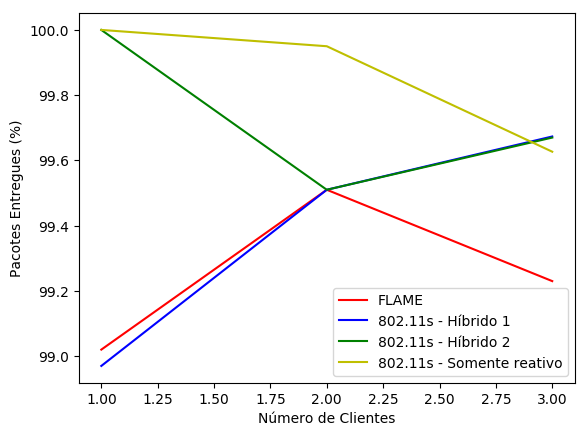
\includegraphics[width=\textwidth]{figuras/pdr_x_numclients_packet512_step25.png}
        \caption{Taxa de entrega de pacotes em função do número de clientes.}
        \label{fig:pdrxnumClients}
    \end{subfigure}
       \begin{subfigure}[b]{0.30\textwidth}
        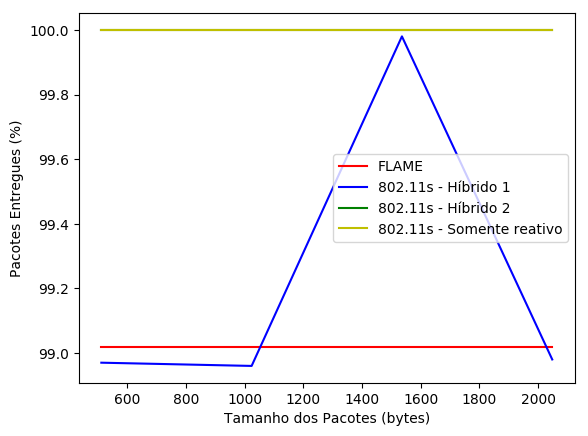
\includegraphics[width=\textwidth]{figuras/pdr_x_packetsize_step25_clients1.png}
        \caption{Taxa de entrega de pacotes em função do tamanho do pacote.}
        \label{fig:pdrxpacketSize}
    \end{subfigure}
       \begin{subfigure}[b]{0.30\textwidth}
        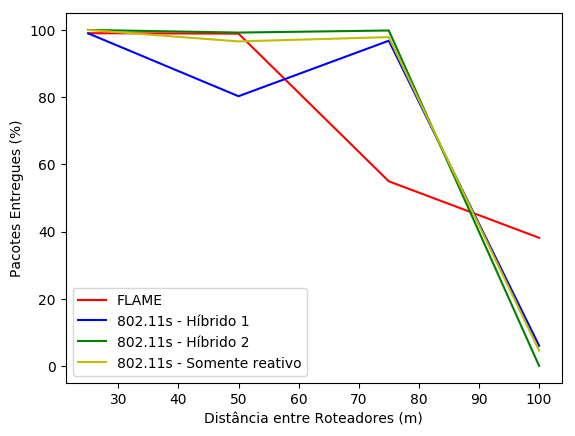
\includegraphics[width=\textwidth]{figuras/pdr_x_stepsize_packet512_clients1.png}
        \caption{Taxa de entrega de pacotes em função da distância entre pares de nós adjacentes.}
        \label{fig:pdrxstepSize}
    \end{subfigure}
\caption{Taxa de Entrega de Pacotes}
\label{fig:pdr}
\end{figure*}

\begin{figure*}[!ht]
\centering
   \begin{subfigure}[b]{0.30\textwidth}
        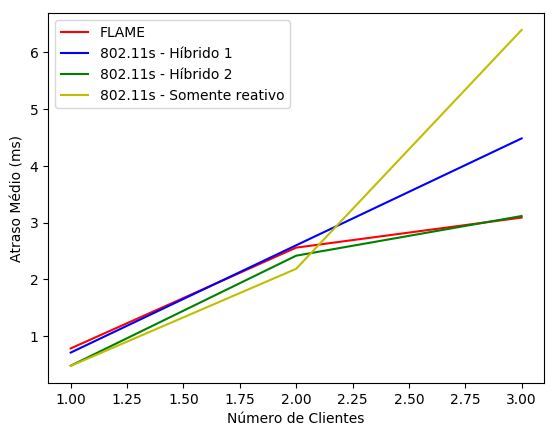
\includegraphics[width=\textwidth]{figuras/avgDelay_x_numclients_packet512_step25.png}
        \caption{Atraso médio em função do número de clientes.}
        \label{fig:avgDelayxnumClients}
    \end{subfigure}
       \begin{subfigure}[b]{0.30\textwidth}
        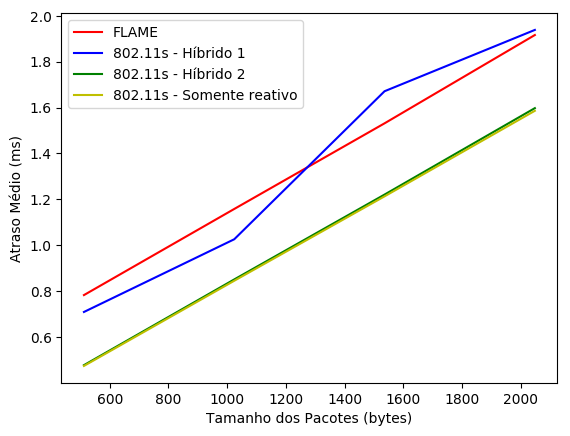
\includegraphics[width=\textwidth]{figuras/avgDelay_x_packetsize_step25_clients1.png}
        \caption{Atraso médio em função do tamanho do pacote.}
        \label{fig:avgDelayxpacketSize}
    \end{subfigure}
       \begin{subfigure}[b]{0.30\textwidth}
        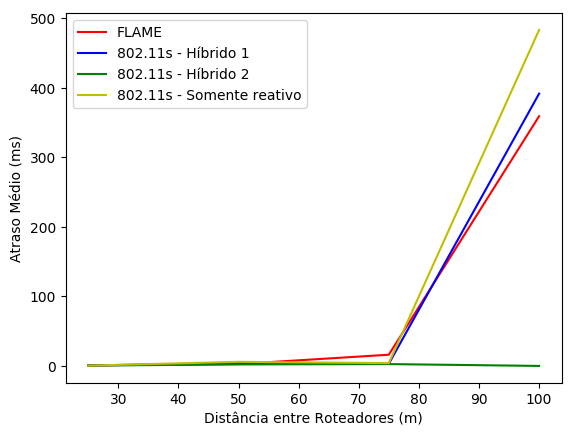
\includegraphics[width=\textwidth]{figuras/avgDelay_x_stepsize_packet512_clients1.png}
        \caption{Atraso médio em função da distância entre pares de nós adjacentes.}
        \label{fig:avgDelayxstepSize}
    \end{subfigure}
\caption{Atraso Médio}
\label{fig:avgDelay}
\end{figure*}

\begin{figure*}[!ht]
\centering
   \begin{subfigure}[b]{0.30\textwidth}
        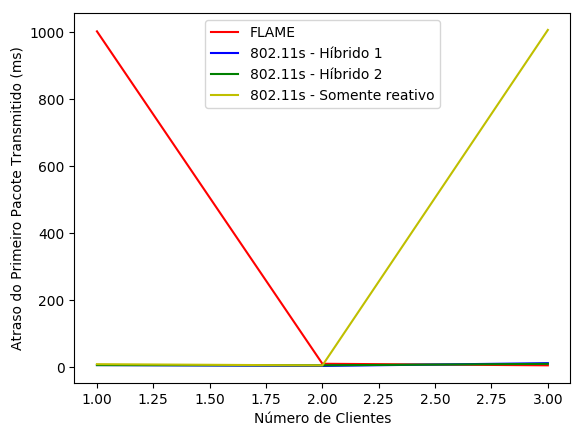
\includegraphics[width=\textwidth]{figuras/firstTransmittedPacketDelay_x_numclients_packet512_step25.png}
        \caption{Atraso do primeiro pacote transmitido em função do número de clientes.}
        \label{fig:firstTransmittedPacketDelayxnumClients}
    \end{subfigure}
       \begin{subfigure}[b]{0.30\textwidth}
        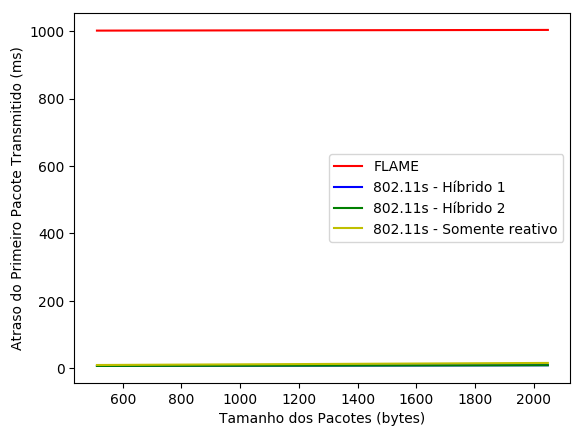
\includegraphics[width=\textwidth]{figuras/firstTransmittedPacketDelay_x_packetsize_step25_clients1.png}
        \caption{Atraso do primeiro pacote transmitido em função do tamanho do pacote.}
        \label{fig:firstTransmittedPacketDelayxpacketSize}
    \end{subfigure}
       \begin{subfigure}[b]{0.30\textwidth}
        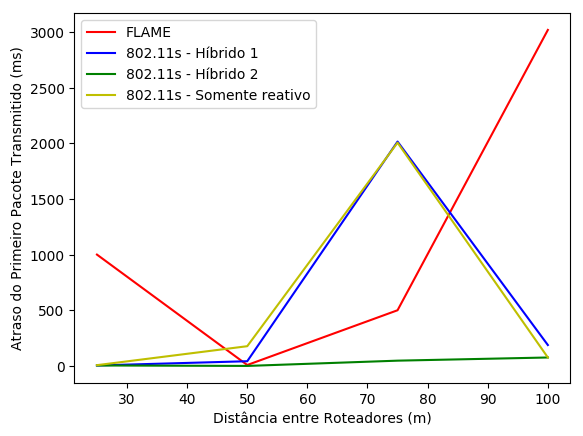
\includegraphics[width=\textwidth]{figuras/firstTransmittedPacketDelay_x_stepsize_packet512_clients1.png}
        \caption{Atraso do primeiro pacote transmitido em função da distância entre pares de nós adjacentes.}
        \label{fig:firstTransmittedPacketDelayxstepSize}
    \end{subfigure}
\caption{Atraso do Primeiro Pacote Transmitido}
\label{fig:firstTransmittedPacketDelay}
\end{figure*}



\section{Conclusões}\label{sec:conc}

Este trabalho realizou uma análise via simulações de redes em malha sem-fio utilizando os protocolos definidos no padrão IEEE 802.11s e o protocolo FLAME. A análise considerada aqui considerou a emissão de tráfego contínuo entre clientes e um servidor dentro de uma topologia quadrada com 9 roteadores cujas posições eram fixas (eram o \textit{backbone} da rede) e verificou o comportamento da taxa de entrega de pacotes, atraso médio e atraso do primeiro pacote transmitido em função do número de clientes, do tamanho do pacote transmitido e da distância entre pares de nós adjacentes. Os resultados obtidos indicam que a escolha do protocolo depende das características do cenário e da aplicação. O protocolo FLAME, consideravelmente menos complexo que o IEEE 802.11s, apresenta uma menor sensibilidade à distância, fazendo com que ele garanta uma maior taxa de entrega de pacotes e um menor atraso médio a maiores distâncias. Isto ocorre devido ao uso das inundações periódicas, que fazem com que parte dos dados transmitidos sigam múltiplos caminhos aleatórios. O FLAME também parece se beneficiar de cenários com múltiplos clientes, dado que os valores de atraso diminuíram. Isto ocorre porque o seu algoritmo obtém informações das próprias transmissões de dados, periodicamente em difusão e mais frequentes que mensagens de controle. No entanto, a menores distâncias, o HWMP, definido pelo IEEE 802.11s, consegue fornecer melhores valores de taxa de entrega de pacotes em qualquer um dos modos. Se existem nós na rede \textit{mesh} por onde circula grande parte do tráfego, o uso de uma árvore com raiz em um dos nós deste conjunto pode ser uma abordagem interessante: a inundação periódica em conjunto com a métrica de \textit{Airtime}, que visa minimizar o tempo durante o qual um quadro é transmitido, permite estabelecer caminhos que oferecem baixos valores de atraso e bom desempenho quanto à entrega de pacotes.

\bibliography{fwc}
\bibliographystyle{IEEEtran}



\end{document}
